\documentclass[10pt]{beamer}

\usepackage{subfig}
\usepackage{amssymb,amsmath,mathtools}
\usepackage{amsfonts,booktabs}
\usepackage{lmodern,textcomp}
\usepackage{color}
\usepackage{tikz}
\usepackage[latin1]{inputenc}
\usepackage{natbib}
\usepackage{multicol}
\usepackage{graphicx}
\usepackage{caption}

\usetheme{Madrid}
\usecolortheme{default}

\title[about the practice]
{About the beamer in the presentation making}
\subtitle{A short story}
\author{Qinghao Hu}


\begin{document}

\frame{\titlepage}

\begin{frame}{The first frame}
  This is some text in the first frame
\end{frame}

\begin{frame}
  \frametitle{Table of Contents}
  \tableofcontents
\end{frame}

\section{item}
\begin{frame}{Same frame title}
  This is a text in second frame. For the sake of showing an example
  \begin{itemize}
    \item Text visible on slide 1
    \item Text visible on slide 2 
    \item Text visible on slide 3
    \item Text visible on slide 4
  \end{itemize}
\end{frame}

\section{Highlighting}
\begin{frame}
  \frametitle{Sample frame title}
  In this slide, some important text will be \alert{highlighted} because it's important.
  Please don't abuse it:
  \begin{block}{Remark}
    Sample Text
  \end{block}

  \begin{alertblock}{Important Theorem} 
    Sample text in red box
  \end{alertblock}

  \begin{exampleblock}{example}
    Sample text in green box, The title of the block is "Example"
  \end{exampleblock}

\end{frame}

\section{Columns}
\begin{frame}
  \frametitle {Two-column slide}
  \begin{columns}
    \column{0.5\textwidth}
    This is a text in first column
    $$E = mc^2$$
    \begin{itemize}
      \item First item
      \item Second item
    \end{itemize}

    \column{0.5\textwidth}
    This text will be in the second column 
    and on a second thoughts, this is a nice looking layout in some cases
  \end{columns}
\end{frame}

\begin{frame}
  \frametitle{Two Images with Captions in Columns}
  \begin{columns}
    \column{0.48\textwidth}
    This is the first change 
    \begin{alertblock}{Concept}
      I'm captured by SS
    \end{alertblock}

    \column{0.48\textwidth}
    \begin{center}
      \begin{figure}
        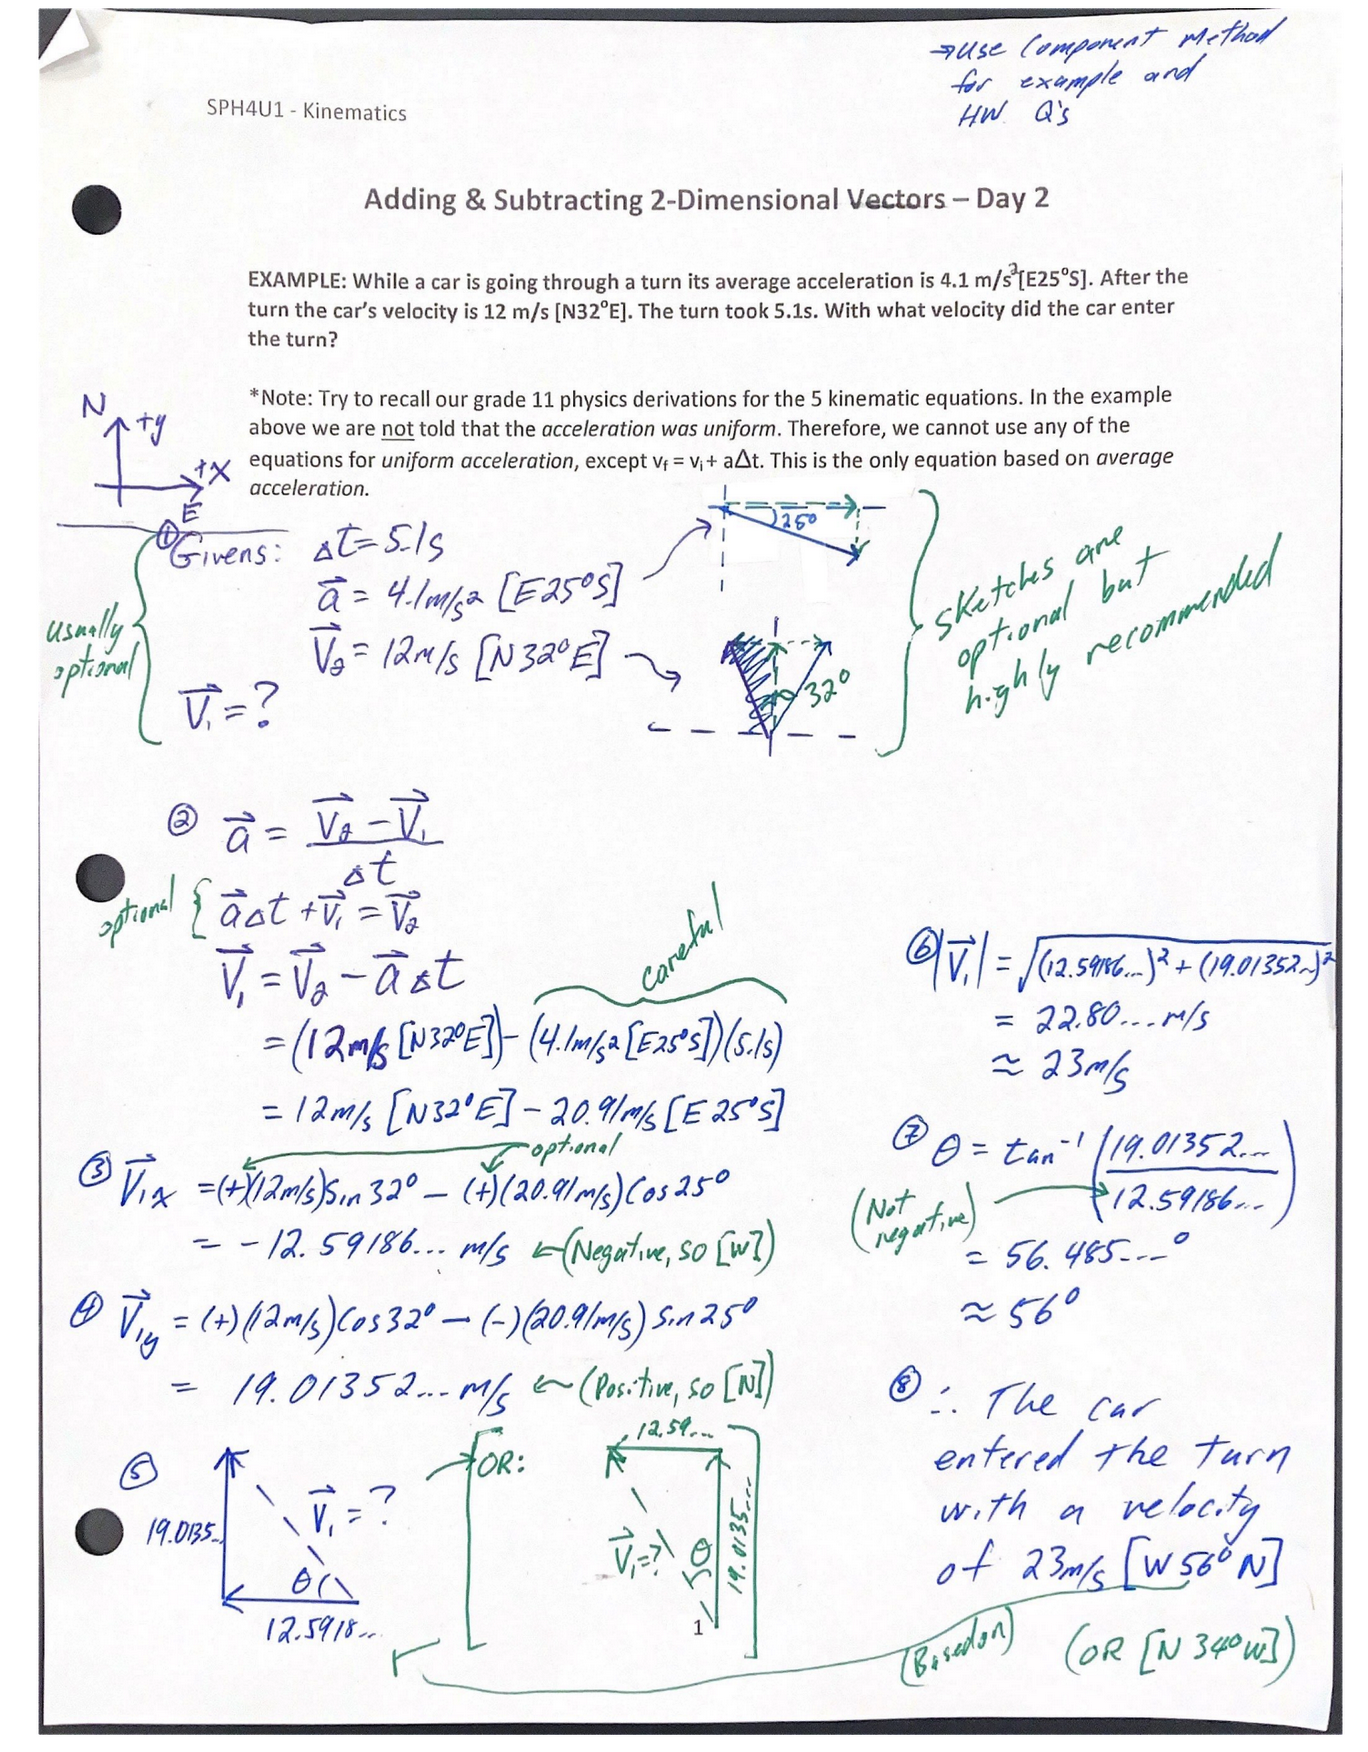
\includegraphics[width=0.7\textwidth]{teacherNote2.png}
        \caption{Teacher's note}
      \end{figure}
    \end{center}
  \end{columns}

\end{frame}

\end{document}

% `\begin{frame}{Image with Description Below}
% \begin{center}
%     \includegraphics[width=0.7\textwidth]{example-image-b.jpg}
%     \captionof{figure}{A descriptive caption for the image}

%     \vspace{0.5cm} % space between image and text

%     This is a short description or explanation related to the image.
%     It can be one or two lines to avoid clutter.
% \end{center}
% \end{frame}
'

% \begin{frame}{Image with Description Below}
% \begin{center}
%     \includegraphics[width=0.7\textwidth]{example-image-b.jpg}
%     \captionof{figure}{A descriptive caption for the image}

%     \vspace{0.5cm} % space between image and text

%     This is a short description or explanation related to the image.
%     It can be one or two lines to avoid clutter.
% \end{center}
% \end{frame}